\documentclass[12pt]{article}
\usepackage{amsmath}
\usepackage{graphicx}
\usepackage{float}
\usepackage{subfig}
\usepackage{epstopdf}
\usepackage[margin=0.8in]{geometry}

%\authorrunninghead{ZHENG ET AL.}

%\titlerunninghead{DNS for Entrainment}

%%\authoraddr{Corresponding author: Y. G. Liu, Brookhaven National Laboratory,
%%Bldg. 815E, Upton, NY 11973-5000, USA. (lyg@bnl.gov)}

%\begin{article}
\newcommand{\Eq}[1]{Eq.~\eqref{#1}} \newcommand{\Fig}[1]{Figure~\ref{#1}}
\newcommand{\Sec}[1]{Sec.~\ref{#1}} \newcommand{\Table}[1]{Table~\ref{#1}}

\begin{document}
\title{A New Particle-Resolved Direct Numerical Simulation Model for Studying Entrainment Processes}
\author{Zheng Gao,
Yangang Liu,
Xiaolin Li}
\maketitle
%\altaffiltext{1}{Department of Applied Mathematics and Statistics, Stony Brook University,
%Stony Brook, NY 11794--3600, USA.}

%\altaffiltext{2}{Brookhaven National Laboratory, Bldg. 815E Upton, NY 11973-5000}

\begin{abstract}
A three dimensional direct numerical simulation (DNS) of the entrainment 
of clear air and its mixing with cloudy air in the decaying and force 
turbulence environment is performed. Since turbulence is a dynamic system 
that is highly sensitive to its initial condition, several initial settings 
have been applied to the simulation and the numerical results were compared 
with each other. It is interesting to see that even with the same cloud 
water fraction, the properties of the thermodynamics and micro-physics are 
highly different especially for the decaying cases. 
The results suggest that the initial shape of cloud filaments should be 
considered as a significant factor in the DNS of cloud entrainment and mixing.   
\end{abstract}

\section{Introduction}
In the past decades, many authors have contributed to the simulation of
turbulent mixing of cloudy and clear air. In Andrejczuk and Grabowski's series work \cite{And04,And06,And09}, an incompressible Boussinesq approximation model, along with vapor mixing ratio and temperature, is proposed to study the cloud-clear air interfacial mixing. Different turbulence kinetic energy (TKE) are used as input parameters at initial time to examine the impact of turbulence intensity on droplet size distribution and mixing homogeneity. The cloud filaments and velocity field are preset to make a heavily idealized initial and boundary condition, while focusing on the details of the evolving flow. 

Kumar and Schumacher in \cite{Kumar11,Kumar12} developed a particle-point DNS to investigate entrainment mixing processes. In their work, a slab-like vapor field is adopted to mimic the supersaturated cloud area and subsaturated environment. The effects of temperature and buoyancy are ignored while an artificial isotropic volume forcing is introduced to maintain the turbulence. Using isotropic artificial forced turbulence is valid for adiabatic cloudy areas, but might be unrealistic at the interface between cloudy and clear air, because the flow in the regions of mixing may not be isotropic due to the negative buoyancy from the droplet evaporation \cite{Vaillancourt00}. In \cite{Kumar14}, the authors extended their previous work to both forced and decaying turbulence, and claimed that the buoyancy due to droplet evaporation played minor role in the mixing for their configuration.

It is interesting to notice that the models and settings in \cite{Kumar11} and \cite{And04} are similar except the geometric shape of the cloud filaments. The cloudy area in \cite{And04} is completely decided by the velocity field of the turbulent flow, thus forming worm-like regions, while a slab-like cloud filament is adopted in \cite{Kumar11}. Since no particular reasons of their choices are given and the effects of cloud shape on the mixing processes are unknown, an investigation on the settings of cloud filaments in DNS becomes significant. In this paper, three different cloud shapes, including the ones in \cite{Kumar11} and \cite{And04}, are tested in the simulation.

The rest of the paper is organized as follows. Section 2 describes
the mathematics model and numerical scheme. In section 3, we give
a brief introduction to the procedure of setting up initial state for simulation. The numerical results and some post-analysis are shown
in section 4. A summary is presented in the last section. 
\section{Particle-Resolved DNS}


\subsection{Dynamical and scalar field}

Following previous DNS, the new DNS is based on the incompressible
Boussinesq approximation whereby the dynamical field is by \cite{And04}:

\begin{subequations}

\begin{equation}
\partial_{t}\mathbf{u}+(\mathbf{u}\cdot\nabla)\mathbf{u}=-\frac{1}{\rho_{0}}\nabla p+\nu\nabla^2 \mathbf{u}+\mathbf{f}\label{eq:NS1}
\end{equation}


\begin{equation}
\nabla\cdot \mathbf{u}=0\label{eq:NS2}
\end{equation}

\end{subequations}

where $\nu$ is the kinetic viscosity, $\rho_{0}$ is the density of
clear air, $\mathbf{u}$ is the velocity field, $p$ is the pressure field. Here $\mathbf{f}$ is the external force imitating the buoyancy effects or the low-wavenumber forcing:
\begin{equation}
\mathbf{f}= \left\{ 
\begin{array}{l}
\mathbf{g}[\frac{T-T_{0}}{T}+0.608(q_{v}-q_{v0})-q_{c}]\\
\mathbf{f}_e
\end{array} 
\right.
\label{eq:source_term}
\end{equation}
where $\mathbf{g}$ is the gravity, $T$ and $q_{v}$ are temperature
and vapor mixing ratio field respectively with the subscript ``$0$''
denoting the reference values; $q_{c}$ is the cloud water mixing
ratio. $\mathbf{f}_e$ is the artificial external force defined in the Fourier space:
\begin{equation}
\mathbf{f}_e = \epsilon_{in}\frac{\mathbf{u}(\mathbf{k},t)}
{\sum_{\mathbf{k}_f\in \kappa}|\mathbf{u}(\mathbf{k}_f,t)|^2}
\sigma_{\mathbf{k},\mathbf{k}_f}
\end{equation}
where $\mathbf{k}$ is chosen from a subset of the wavenumber space $\kappa$ containing a few wavevectors, $\epsilon_{in}$ is the input energy rate. $\delta_{k,k_f}$ is a delta function. Therefore, statistics stationary homogeneous turbulence 
can be obtained in DNS by forcing the low-wavenumber modes.

The temperature and vapor mixing ratio are solved from the following
equations (\cite{Kumar11}):

\begin{equation}
\partial_{t}T+(\mathbf{u}\cdot\nabla)T=\frac{L_{h}}{c_{p}}C_{d}+\mu_{T}\nabla^{2}T\label{eq:Temp}
\end{equation}
\begin{equation}
\partial_{t}q_{v}+(\mathbf{u}\cdot\nabla)q_{v}=-C_{d}+\mu_{v}\nabla^{2}q_{v}\label{eq:Vapor}
\end{equation}


In the above equations, $L_{h}$ is the latent heat of water vapor condensation,
$c_{p}$ is the specific heat at constant pressure, $\mu_{T}=\mu_{v}$ are
the molecular diffusivity for temperature and water vapor, respectively
and assumes to be equal. The parameter $C_{d}$ is the condensation
rate defined as the rate of exchanging water between liquid and vapor
per unit time, and is computed in the DNS by:

\begin{subequations}

\begin{equation}
C_{d}(\mathbf{X},t)=\frac{d(m_{l}(\mathbf{X},t))}{m_{a}dt}=\frac{4\pi\rho_{l}K}{\rho_{0}a^{3}}\Sigma_{i=1}^{n}S(\mathbf{X}_{i},t)R_{i}(t)\label{eq:CondRate}
\end{equation}


where $K$ is a function of temperature and pressure given by:

\begin{equation}
K=1/[(\frac{L_{h}}{R_{v}T}-1)\frac{L_{h}\rho_{l}}{C_{T}T}+\frac{\rho_{l}R_{v}T}{De_{s}(T)}]\label{eq:CondCoeff}
\end{equation}


where $R_{v}$ is the individual gas constant, $T$ is the temperature,
$C_{T}$ is the coefficient of thermal conductivity, $e_{s}(T)$ is
the saturation vapor pressure. The supersaturation $S(X,t)$ is calculated
directly from the water vapor and temperature by using the following
equation

\begin{equation}
S(\mathbf{X},t)=\frac{q_{v}(\mathbf{X},t)}{q_{v,s}(\mathbf{X},t)}-1\label{eq:Supersat}
\end{equation}


\end{subequations}

where $q_{v}(\mathbf{X},t)$ is the vapor mixing ratio from equation (\ref{eq:Vapor})
and $q_{v,s}$ is the saturated water vapor mixing ratio. The droplets
will grow with positive supersaturation while shrink with negative
one.

\begin{equation}
q_{c}(\mathbf{X},t)=\frac{4\pi\rho_{l}}{3\rho_{0}a^{3}}\sum_{i=1}^{n}R_{i}^{3}(t)\label{eq:cloud_water}
\end{equation}


where $a$ is the size of a grid cell, $n$ is the number of droplets
in the grid cell. $\rho_{l}$ and $\rho_{0}$ are the density of water
droplets and the air. $R_{i}(t)$ is the radius of the $i$th droplet
inside a grid cell.


\subsection{Droplet growth and motion}

To describe the motion and condensation of droplets, we use

\begin{equation}
R(t)\frac{R(t)}{dt}=K\cdot S(\mathbf{X},t)\label{eq:Radius}
\end{equation}


\begin{equation}
\frac{d\mathbf{X}(t)}{dt}=\mathbf{V}(t)\label{eq:Coords}
\end{equation}


\begin{equation}
\frac{d\mathbf{V}(t)}{dt}=\frac{1}{\tau_{p}}[\mathbf{u}(\mathbf{X},t)-\mathbf{V}(t)]+\mathbf{g}\label{eq:Velocity}
\end{equation}


Here $R(t)$ is the radius of a single droplet, $\mathbf{X}(t)$ is the position
coordinate and $\mathbf{V}(t)$ is the velocity, $\mathbf{g}$ is the gravitational constant. $\tau_{p}=2\rho_{l}R^{2}/(9\rho_{0}\nu)$ is the finite
particle response time. The particle response time measures the droplet
inertial effects; when $\tau_{p}$ is set to be zero, equation (\ref{eq:Velocity}) becomes $\mathbf{V}(t)=\mathbf{u}(\mathbf{X},t)$, which implies that the droplets will exactly follows the turbulence flows. The last term in equation (\ref{eq:Velocity}) is the sedimentation term that accounts for the effect of gravity on droplets motion. Equation (\ref{eq:Velocity}) is appropriate if the Reynolds number based on the relative velocity between the particle and fluid is significantly less than one \cite{Eaton94}. The particle
diameter is also assumed to be smaller than the Kolmogorov microscale
$\eta$, the smallest length scales of the turbulent flow field. During
condensation, direct interactions between droplets are negligible because
their sizes are too small comparing with the average distance between
two droplets.

\subsection{Numerical Implementation}
Up to now the most successful direct numerical simulations of homogeneous 
turbulence were performed with pseudo-spectral methods due to its 
superior accuracy \cite{Rogallo81,Orszag72}. In recent years, pseudo-spectral 
method has been extensively applied to the numerical study of cloud 
entrainment problem in turbulent flows \cite{And04,Celani05,Kumar11}. However, the standard pseudo-spectral method has some severe restrictions. 
As claimed in \cite{Kumar11}, the spectral method requires a smooth initial condition to avoid the Gibbs phenomenon. This artificial initial condition is not realistic or physical, thus has potential to bring some imperceptible errors during the simulation. Moreover, the spectral method requires periodic boundary condition in each direction and cannot be applied to flows that require a non-periodic, physical boundary condition. To be flexible enough to deal with various initial profiles with sharp cloudy-clear air interfaces as well as applying different boundary conditions in the future, equations (\ref{eq:NS1})--(\ref{eq:Vapor}) are solved by finite difference method coupled with WENO (weighted essentially non-oscillatory) scheme \cite{WENO96}, which has the capability of dealing with discontinuity without causing numerical overshoots at sharp interfaces. Droplets position (\ref{eq:Coords}) and motion (\ref{eq:Velocity}) are solved by implicit Euler method in consideration of efficiency and stability. The time step size is adaptive to satisfy the Courant-–Friedrichs-–Lewy (CFL) condition. Parallel computing techniques are implemented with MPI library to increase the computational speed.

The numerical domain is set to be $0.512m^{3}$ with periodic boundary
in all directions. The computational grid is $256^{3}$, thus
giving the corresponding grid length of $2mm$. This grid size falls
between the droplet distance of $1cm$ vital for turbulence-microphysics 
interactions and the typical Kolmogorov length of $1mm$.

\section{Effects of sedimentation on preferential concentration }
Clustering of inertial particles has been extensively studied via both 
experiments and numerical simulations \cite{Sundaram97, Reade2000}, but the sedimentation effects on the clustering are poorly understood. In this section, a series of numerical test are performed by gradually increasing the 
gravity force and calculate the corresponding clustering index \cite{Vaillancourt02} with
\begin{equation}
C_L = \hat{V}_L(n)/V_L(n)-1
\label{eq:cluster_index}
\end{equation}
where $\hat{V}_L(n)$ is the measured variance of the number density and $V_L(n)$ is the mean concentration of droplets.
From the history of the clustering index \Fig{fig:gravity_cluster}, one can clearly tell that the clustering index increase at the beginning stage due to the strong turbulence fluctuation and then decrease as the turbulence decaying. Another observation is that strong gravity force leads to weak preferential concentration results. The conclusion also holds for the forced turbulence.
\begin{figure}[H]
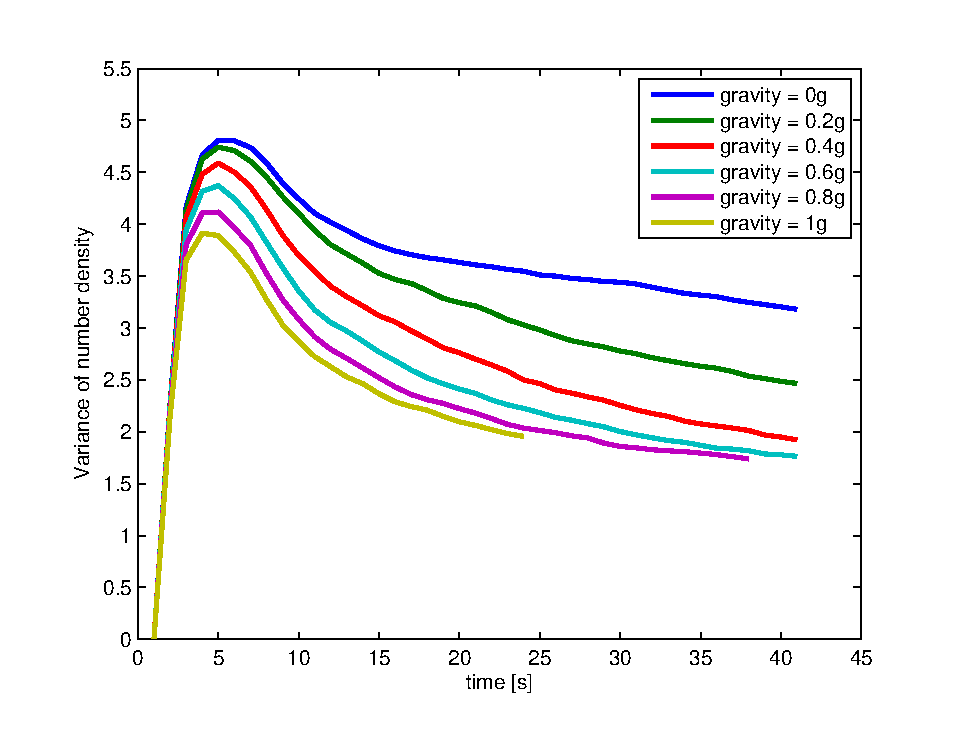
\includegraphics[width=0.45\textwidth]{Figures/gravity_time_decay}
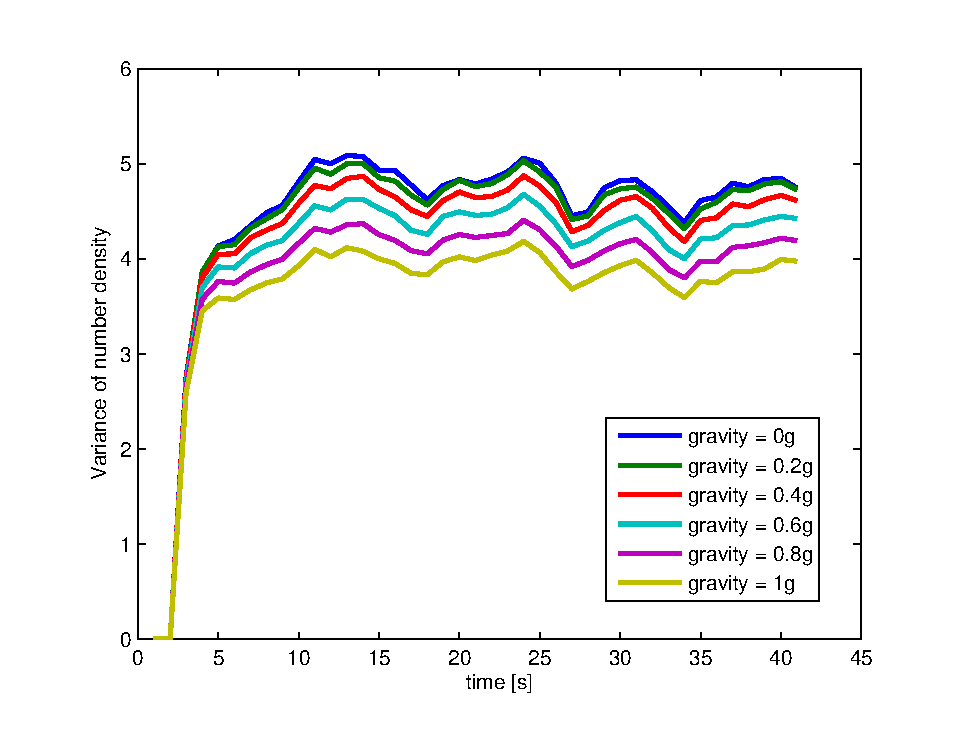
\includegraphics[width=0.45\textwidth]{Figures/gravity_time_force}
\caption{Time evolution of clustering index with different sedimentation term in decaying turbulence (see left) and 
forced turbulence (see right figure).}
\label{fig:gravity_cluster}
\end{figure}

\section{Simulation of entrainment and mixing processes}

Depending on the mixing scenario (the homogeneity of mixing), the
droplets will evolve in quite different ways. In the extremely homogeneous mixing scenario, the number of droplets does not change while the mean radius decreases. In the extremely inhomogeneous mixing scenario, some droplets in the cloud completely disappear while the others remain the mean radius. This mixing of clear and cloudy air is often quantified by the Damkohler number:

\begin{equation}
Da=\frac{\tau_{mix}}{\tau_{react}}\label{eq:DaNumber}
\end{equation}


here $\tau_{mix}$ is the time scale for an eddy of size $l_E$ and is defined as:

\begin{equation}
\tau_{mix}=(\frac{l_E^{2}}{\varepsilon})^{1/3}\label{eq:Tmix}
\end{equation}

$\tau_{react}$ is the time for complete chemical reaction, which often given by the evaporation time scale in the cloud physics literature:
\begin{equation}
\tau_{e}=\frac{R_{m}^{2}}{-KS}\label{eq:Tevap}
\end{equation}
where $R_{m}$ is the mean radius of a droplets group and $K$ is defined
by (\ref{eq:CondCoeff}), $S$ is the averaged supersaturation over
the cloud-free part of the computational domain. In general, $Da\ll1$ corresponds to the homogeneous mixing while $Da\gg1$ is the inhomogeneous one. The real entrainment and mixing process has a $Da$ number often between
these two limits.

In spite of popularity, this approach has a shortcoming:
the value of $l_E$ used in (\ref{eq:Tmix}) is ambiguous. To overcome this difficulty, Lehmann(\cite{Lehmann09}) introduced the concept of transition length $l^{*}$, at which the mixing transits from inhomogeneous to homogeneous:
\begin{equation}
l^{*}=\varepsilon^{1/2}\tau_{react}^{3/2}\label{eq:TransL}
\end{equation}
where the reaction time $\tau_{react}$ is defined as either the time when the droplets have completely evaporated or the time at which the averaged supersaturation $S>-0.005$. The $\tau_{react}$ is computed by solving the following ordinary differential equation with instantaneous volume mean radius and mean supersaturation as the initial condition:
\begin{equation}
\frac{dR_{m}}{dt}=K\frac{S}{R_{m}}\label{eq:DiffR}
\end{equation}

\begin{equation}
\frac{dS}{dt}=-BR_{m}S\label{eq:DiffSuper}
\end{equation}
where $B$ is a function of pressure and temperature, whose specific definition can be found in \cite{Chunsong11}. With transition length $l^{*}$, a dimensionless number called transition scale number was introduced in \cite{Chunsong13} and defined as the ratio of $l^{*}$ and Kolmogorov length scale $\eta$:

\begin{equation}
N_{L}=\frac{l^{*}}{\eta}\label{eq:NL}
\end{equation}

To characterize the microphysical properties of the mixing, the $\langle r^3\rangle -N_d$ diagram (volume mean radius versus number density) was introduced in \cite{Burnet07} and has been widely applied to study the homogeneous/inhomogeneous entrainment-mixing process. With $\langle r^3\rangle -N_d$ diagram, one can predict the extremely homogeneous mixing line at different supersaturation (\cite{Lehmann09,Kumar14}). Another useful quantity is the homogeneous mixing degree $\alpha$:

\begin{equation}
N=N_{a}(\frac{q_l}{q_{l_0}})^{\alpha}\label{eq:alpha}
\end{equation}
where $N_{a}$ and $q_{l_a}$ are the adiabatic value of number density and liquid water mixing ratio, and $N$ and $q_{l}$ are the instantaneous values in the sample boxes.

The entrainment and mixing process can be simulated via placing the supersaturated cloud filaments in the turbulent environment of low humidity. In this section, we will give a detailed description of the initial configurations of the velocity field, vapor mixing ratio, temperature and droplets. 

\subsection{Initial velocity field}

Since turbulence is sensitive to the initial condition and we expect
to obtain a statistically stationary state in a short time before injecting the droplets, an artificial initial velocity field is constructed in Fourier space and then transformed to physical space. Following the procedure proposed in \cite{Rogallo81}, one can generate a solenoidal isotropic velocity field with prescribed energy spectrum \cite{Rosales05}
\begin{equation}
E(k) = \frac{16}{\sqrt{\pi/2}}\frac{u_0^2k^4}{k_0^5}\exp(-\frac{2k^2}{k_0^2})
\end{equation}
where $u_0^2$ is the initial r.m.s. velocity, and $k_0$ is the wavenumber at which the maximum of $E(k)$ occurs. By controlling the value of $u_0$ and $k_0$, we can start from velocity fields with very different intensities and energy distributions.

Following quantities are defined to characterize the turbulence field. 
The dissipation rate is defined as $\varepsilon=2\nu(\frac{\partial u_{i}}{\partial x_{j}}+\frac{\partial u_{j}}{\partial x_{i}})^{2}$,
$\nu$ is the kinematic viscosity of air $1.5\times10^{-5}m^{2}s^{-1}$, and $u_{rms}$
is the root mean square of velocity fluctuation. $\tau_{\eta}$ is
the Kolmogorov time scale defined as $(\nu/\varepsilon)^{1/2}$. $\tau_L$
is the eddy turnover time, estimated by $L_x/u_{rms}$
where $L_x$ is the domain size.

\begin{figure}[H]
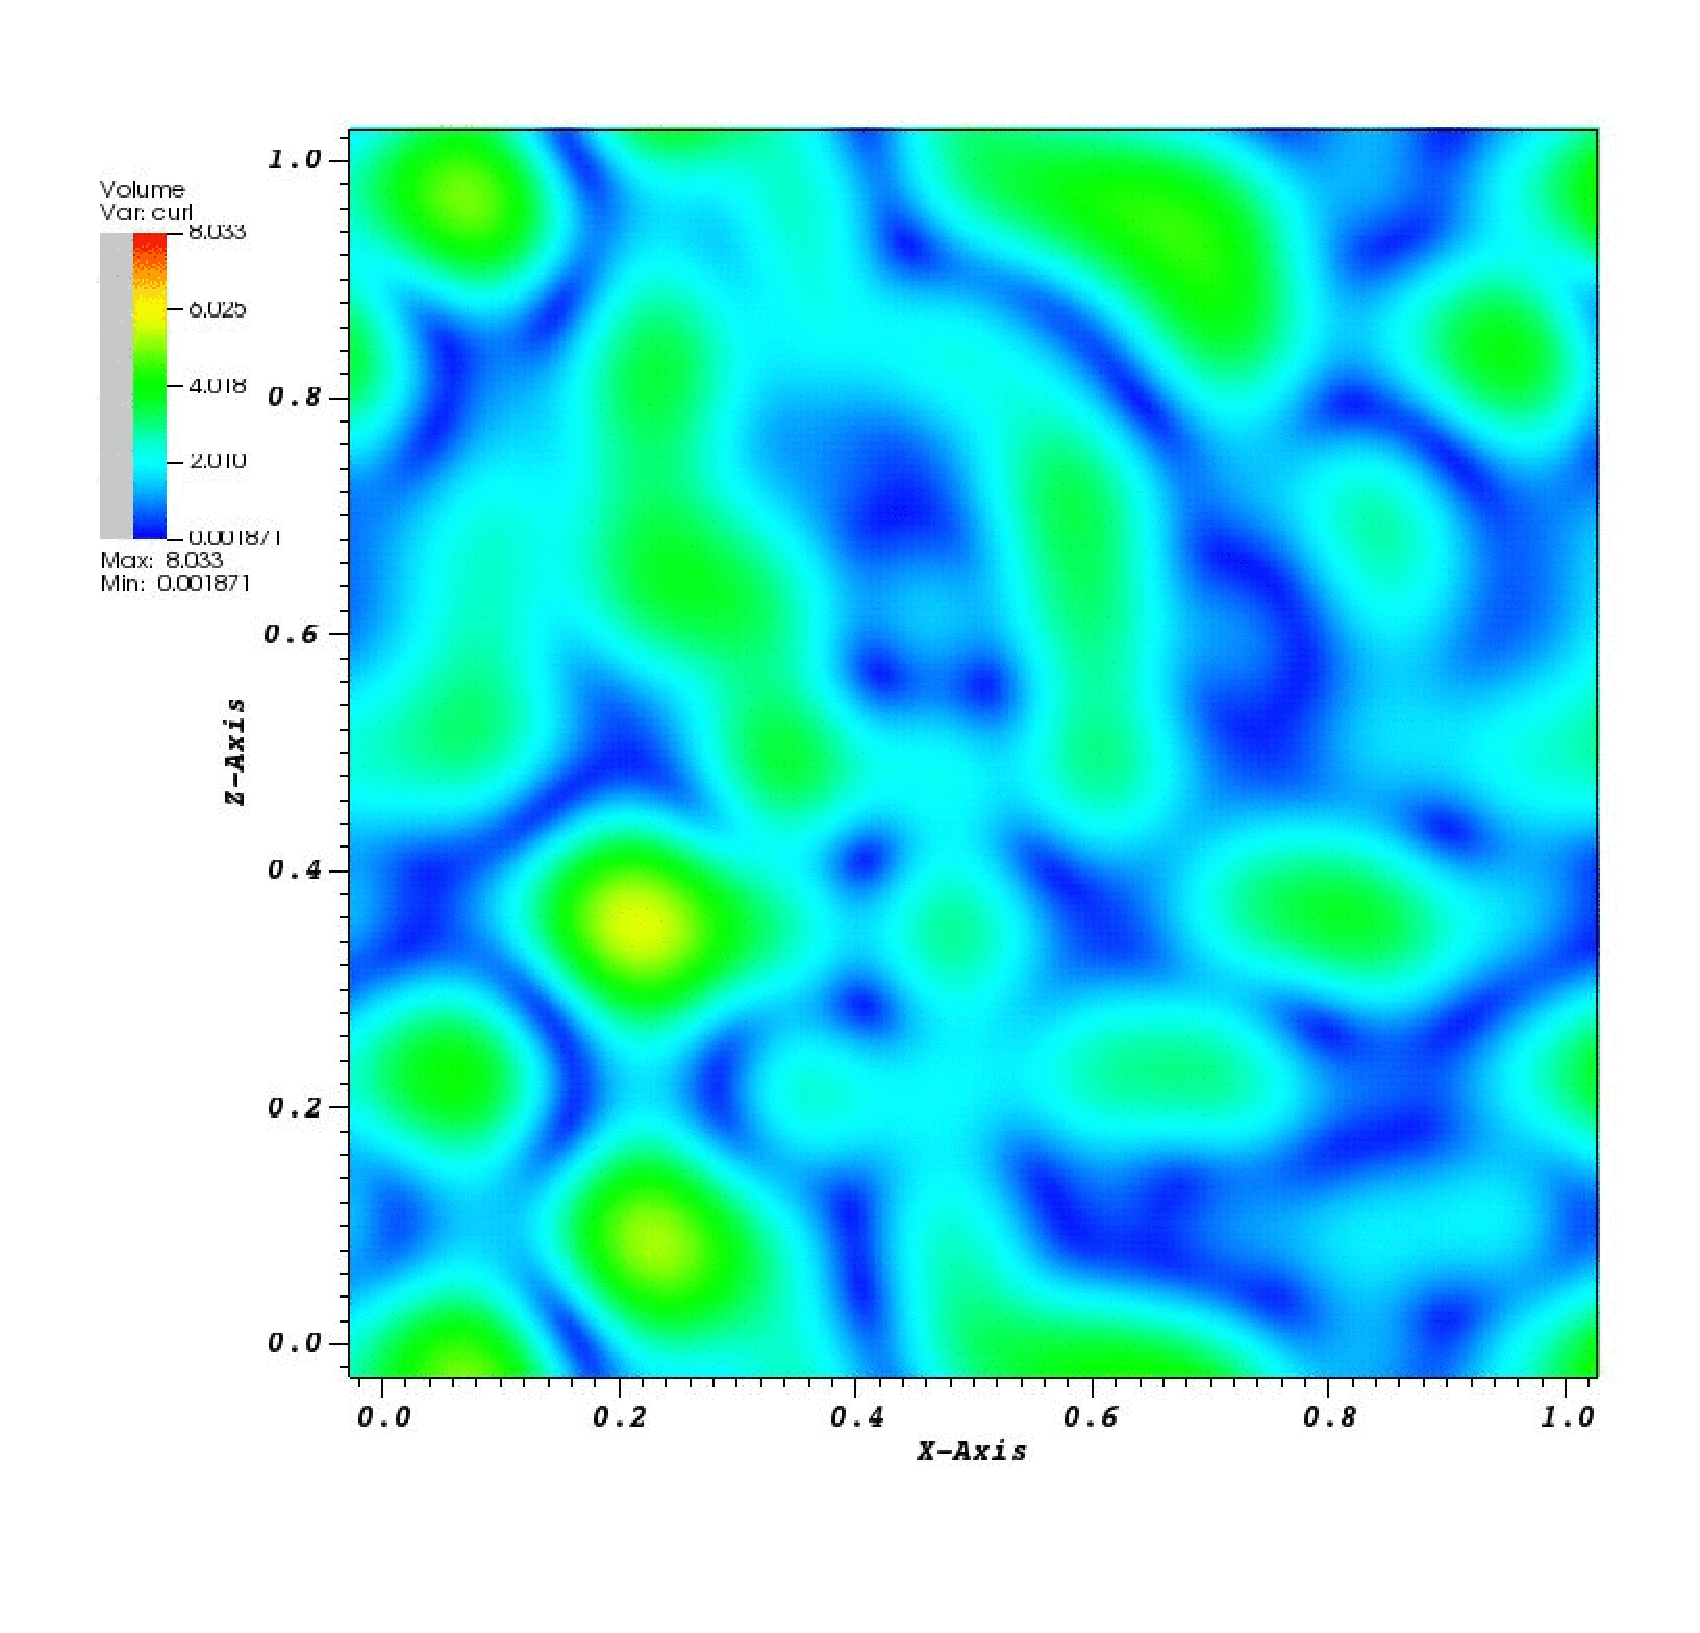
\includegraphics[width=0.48\textwidth]{Figures/vortex-0}
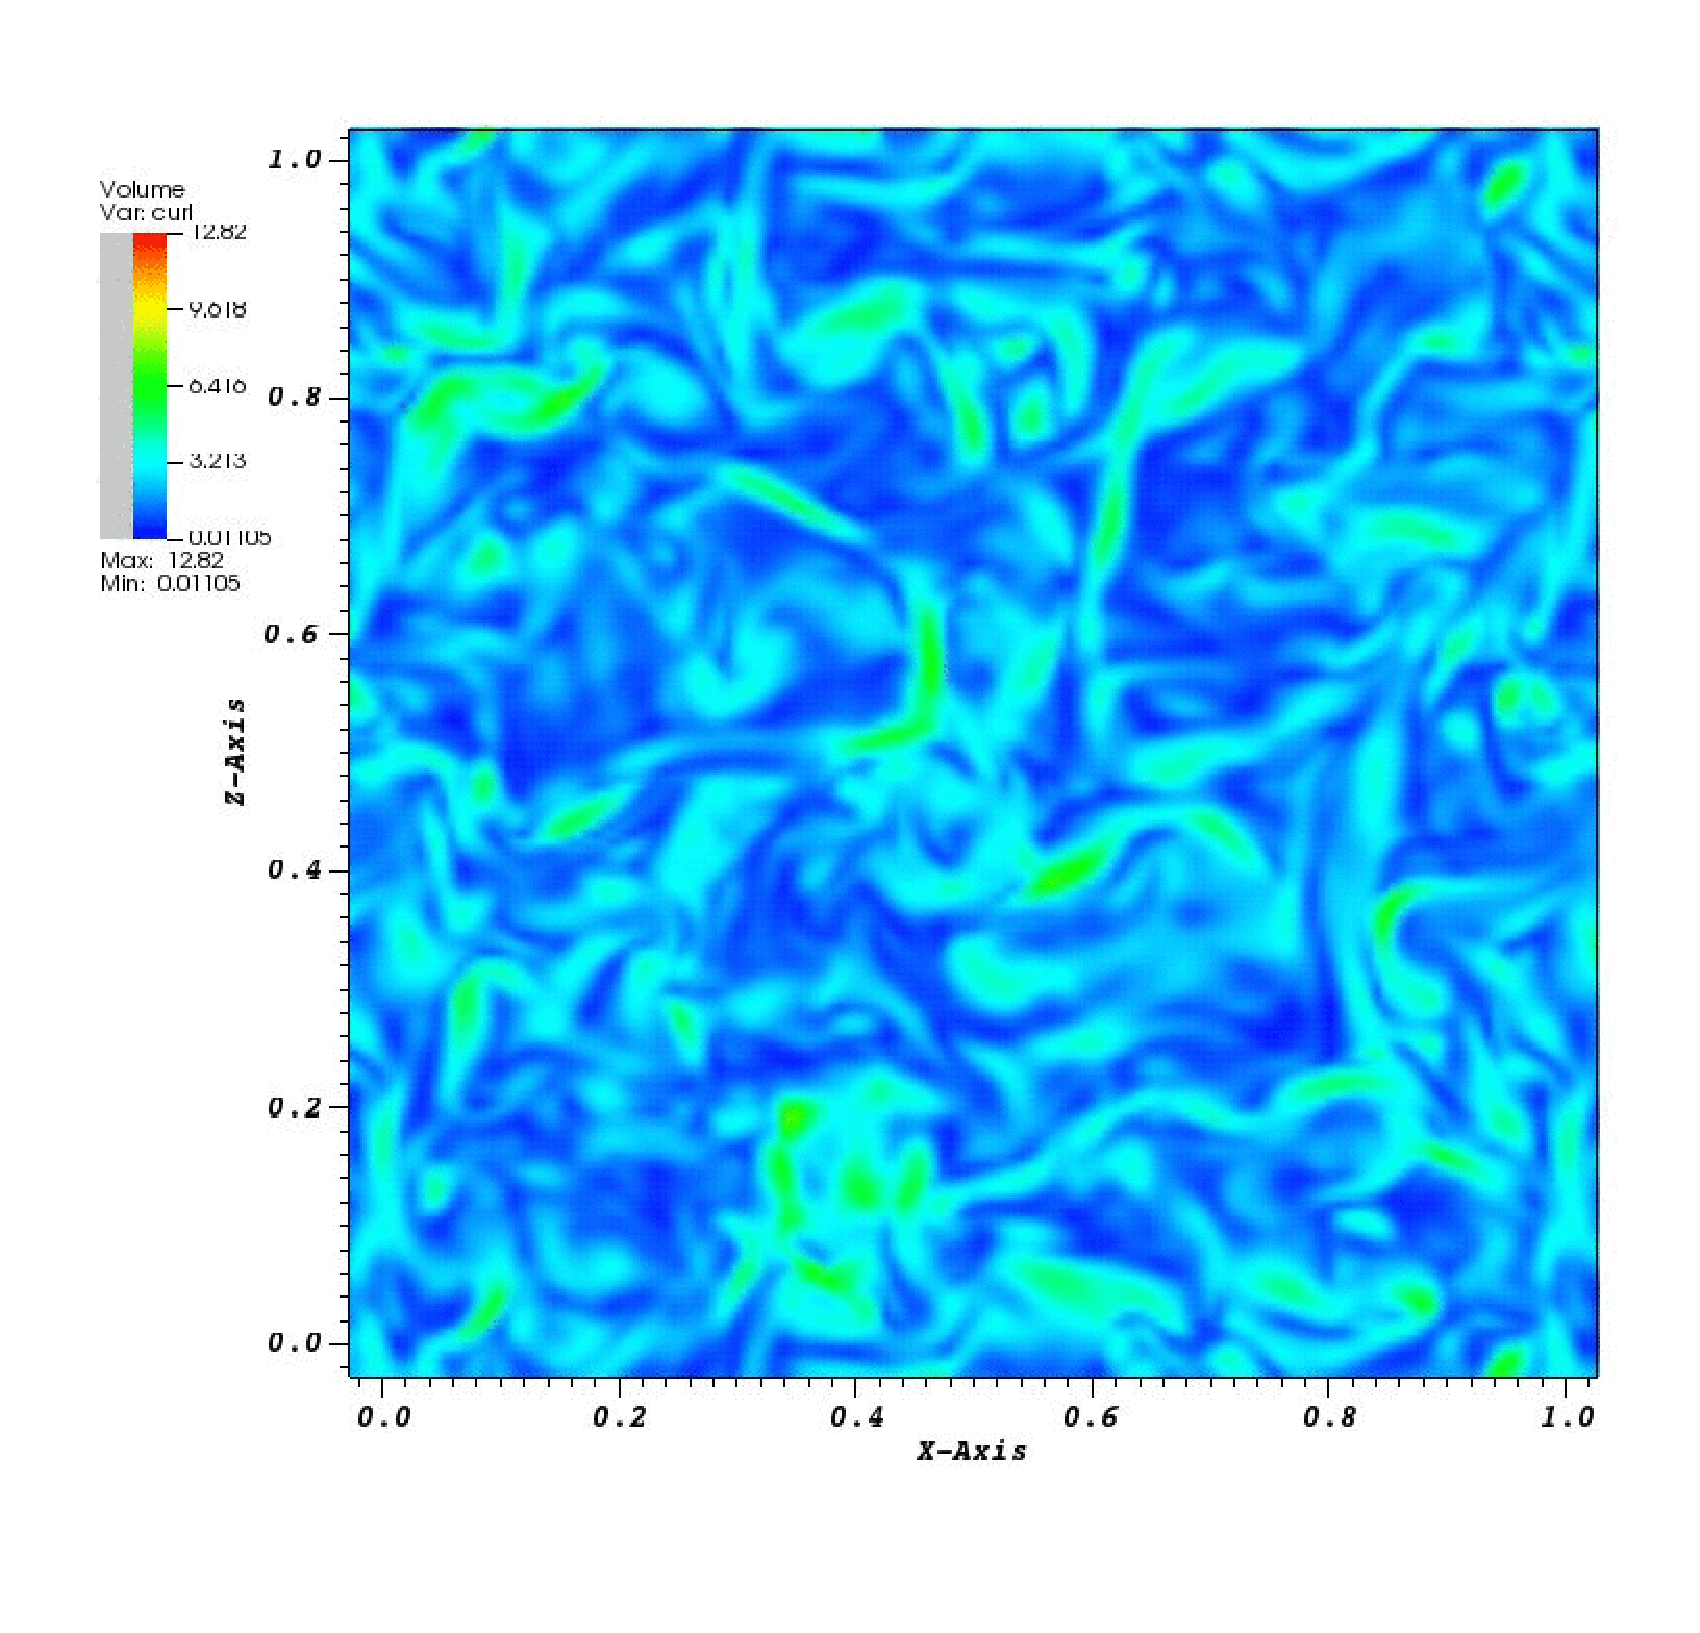
\includegraphics[width=0.48\textwidth]{Figures/vortex-1}

\caption{initial and final enstrophy field in x-z cross-sectional
plane defined as $\varepsilon(\mathbf{u}) = 0.5(\nabla\times\mathbf{u})^2$\label{fig:enstrophy}}
\end{figure}

\subsection{Initial vapor mixing ratio and temperature}
A straightforward way to initialize the vapor mixing ratio is to divide the computational domain into the regions of cloudy and clear air, then assign different values to each subdomain. By specifying the initialization functions, various initial profile for the vapor mixing ratio can be achieved. For example, in \cite{And04}, the function is defined according to the sign of the first component of velocity $\mathbf{u}$. This configuration will be referred to as case 1. In \cite{Kumar11}, the author used an artificial continuous function to construct a slab-like cloud filament. This situation can also be approximated by a simple discontinuous function and will be referred to as case 2. Rotating the slab-like cloud clockwise by $90$ degree, we obtain case 3. The initial vapor content profile for three cases are given by equations (\ref{case1}--\ref{case3}) and illustrated in figure (\ref{fig:v_field_case123}).
\begin{equation}
\mbox{case 1: } q_v(\mathbf{x},t=0) = 
\begin{cases} 
q_v^{max}, & u(\mathbf{x}) > 0\\
q_{v,e}, & u(\mathbf{x}) \le 0
\end{cases}\label{case1}
\end{equation}

\begin{equation}
\mbox{case 2: } q_v(x,t=0) = 
\begin{cases} 
q_v^{max}, & (L-d)/2 \le x < (L+d)/2\\
q_{v,e}, & \mbox{elsewhere}
\end{cases}\label{case2}
\end{equation}

\begin{equation}
\mbox{case 3: } q_v(z,t=0) = 
\begin{cases} 
q_v^{max}, & (L-d)/2 \le z < (L+d)/2\\
q_{v,e}, & \mbox{elsewhere}
\end{cases}\label{case3}
\end{equation}
where $q_v^{max}$ is maximum amplitude of $q_v$, which exceeds $q_{v,s}$ by $2\%$, and $q_{v,e}$ is the vapor mixing ratio of the clear air. $L$ is the length of computational domain, and $d = L/2$ is the width of the cloud slab. 
\begin{figure}[H]
\includegraphics[width=1.0\textwidth]{Figures/v_field_case123}
\caption{Cross sectional view of the initial vapor mixing ratio for different cases: case 1, 2, 3 from left to right. The cloudy part occupies about half of the computational domain.\label{fig:v_field_case123}}
\end{figure}

Finally, the temperature field is initialized by imposing the neutral buoyancy restriction:
\begin{equation}
T(x,t = 0) = T_0 - 0.608T_0[q_v(x,t = 0) - q_{v0}]
\end{equation}
where the reference values are defined by volume averages $T_0 = \langle T(t=0)\rangle_V$ and $q_{v0} = \langle q_v(t=0)\rangle_V$. This condition implies that neither the vapor mixing ratio nor temperature would contribute to the initial buoyancy.  
\subsection{Initial droplets}

The cloud water is distributed to approximately $10^{7}$ number of droplets, which have the same sizes and are uniformly placed in the cloudy region at time $0s$. After the turbulence reaches a steady state in a short time, the droplets will be freed to move and change their sizes according to the physics law. A droplet with zero radius will be immediately removed from the computational domain and will not contribute to any statistical results. Some important quantities for initial condition are summarized in table~\ref{tb:parameters}.
\begin{table}
\begin{tabular}{llllll}
\hline\hline
Quantity & Symbol & Value & Quantity & Symbol & Value\tabularnewline
\hline
Grid points & $N$ & $256$ & Droplet radius & $R_{0}$ & $15\mu m$\tabularnewline
\hline 
Box length & $L$ & $0.512m$ & Environ supersat & $S_{e}$ & $-0.99$\tabularnewline
\hline 
Grid size & $a$ & $0.002m$ & Cloud supersat & $S_{c}$ & $0.02$\tabularnewline
\hline 
Viscosity & $\nu$ & $1.5\times10^{-5}m^{2}s^{-1}$ & Number density& $N_{c}$ & $153cm^{-3}$\tabularnewline
\hline 
Dissip rate& $\epsilon$ & $2.0\times10^{-3}m^{2}s^{-3}$ & Eddy turnover time & $\tau_{L}$ & $4.27s$\tabularnewline
\hline 
Dissip length& $\eta$ & $10^{-3}m$ & Evaporation time & $\tau_{evap}$ & $2.09s$\tabularnewline
\hline 
Dissip time& $\tau_{\eta}$ & $0.087s$ & Reaction time & $\tau_{react}$ & $6.36s$\tabularnewline
\hline 
\end{tabular}
\caption{Initial conditions}\label{tb:parameters}
\end{table}
 
\section{Numerical Results}
The main goal in this paper is using numerical simulation to study
the entrainment and mixing process which often occurs near the cloud-clear air interface. In this section, some principal results are presented, including thermodynamics, microphysics.

\subsection{Thermodynamics}
The $q_{max}$ in each case is set to be $3.95g/kg$ and the $q_{v,e}$ is $0.03g/kg$. The simulation is terminated when droplets completely evaporate or the supersaturation field becomes nearly uniform ($std<0.0002$). Figure \ref{fig:therm_dynam} (top-left) displays the temporal evolution of the variance of vapor mixing ratio fluctuations, which is defined as:
\[
q'_v(\mathbf{x},t) = q_v(\mathbf{x},t)-\langle q_v(t)\rangle_V
\]
and the same definition holds for the temperature. An observation for the cases of decaying turbulence (case D1, D2, D3) is that, in spite of similar configuration with D2, case D3 has stronger fluctuations in temperature and faster evaporation process. This can be explained by the fact that the sedimentation effects accelerate the exchange of heat and water between cloudy and clear air in the vertical direction. We also observed that, the mixing of D1 is faster than D2 and D3 since it can be regarded as an intermediate process in D2 or D3. However, this difference becomes smaller in the forced turbulence as the motion of particles is dominated by the external forcing which are the same for F1, F2 and F3.
\begin{figure}[H]
\includegraphics[width=0.48\textwidth]{Figures/vap_var}
\includegraphics[width=0.48\textwidth]{Figures/temp_var}\\
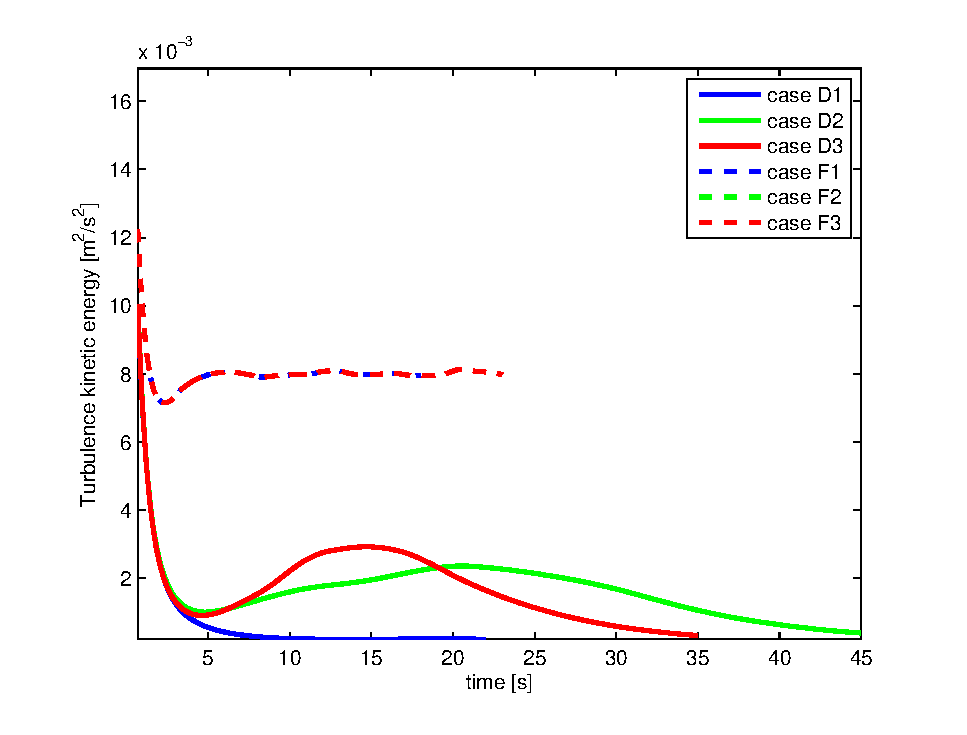
\includegraphics[width=0.48\textwidth]{Figures/tke}
\includegraphics[width=0.48\textwidth]{Figures/num_tot}
\caption{Thermodynamics of three cases, from left to right, up to bottom, are variance of vapor mixing ratio, variance of temperature, turbulence kinetic energy and total droplets number.\label{fig:therm_dynam}}
\end{figure}

\subsection{Microphysics}
The radius distributions for case 1, 2 ,3 in both decaying and forced turbulence are displayed in \Fig{fig:rad_distri}. At the initial stage, some droplets enter into the clear air and expand their size distribution. As mixing going on, since the environment becomes unsaturated and homogeneous, the distribution starts to shift to zero. It continues approaching to zero until completely evaporation happens or the background environment becomes saturated. 
In the \Fig{fig:rad_distri}, an important observation is that case D1, D2 and D3 are quite different in both reaction time and size distribution. However, by substituting the buoyancy by external force, these difference almost disappear. This demonstrates that the difference is caused by the buoyancy term in \Eq{eq:source_term}. In specific, the buoyancy plays as a source of kinetic energy, so as to accelerate the motion of fluid field.
\begin{figure}[H]
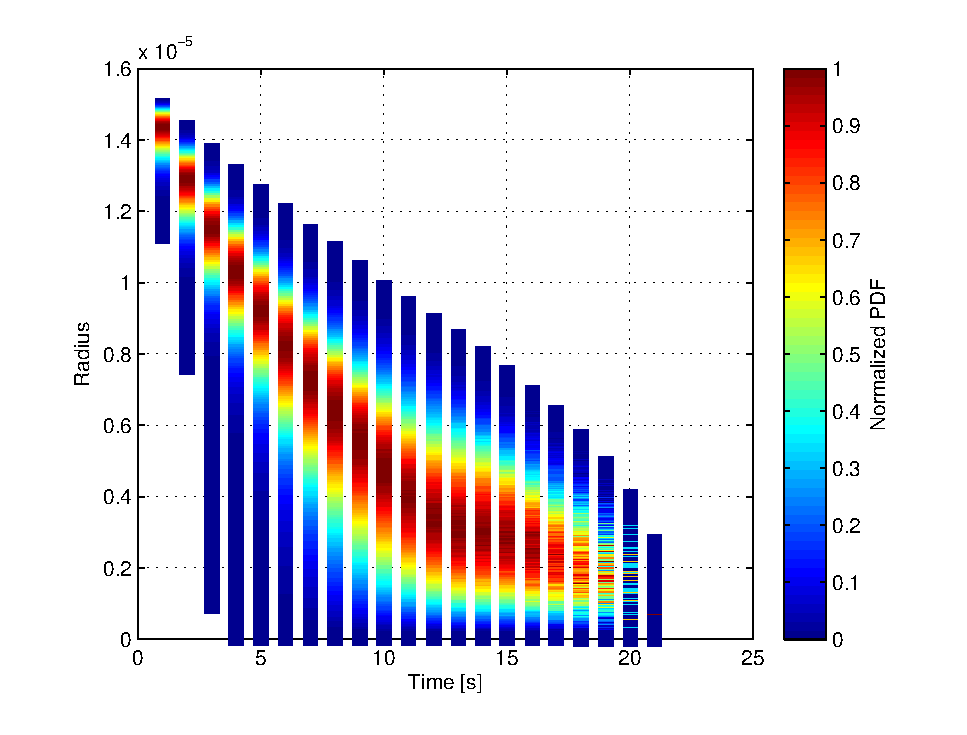
\includegraphics[width=0.48\textwidth]{Figures/pdf_radius_d1}
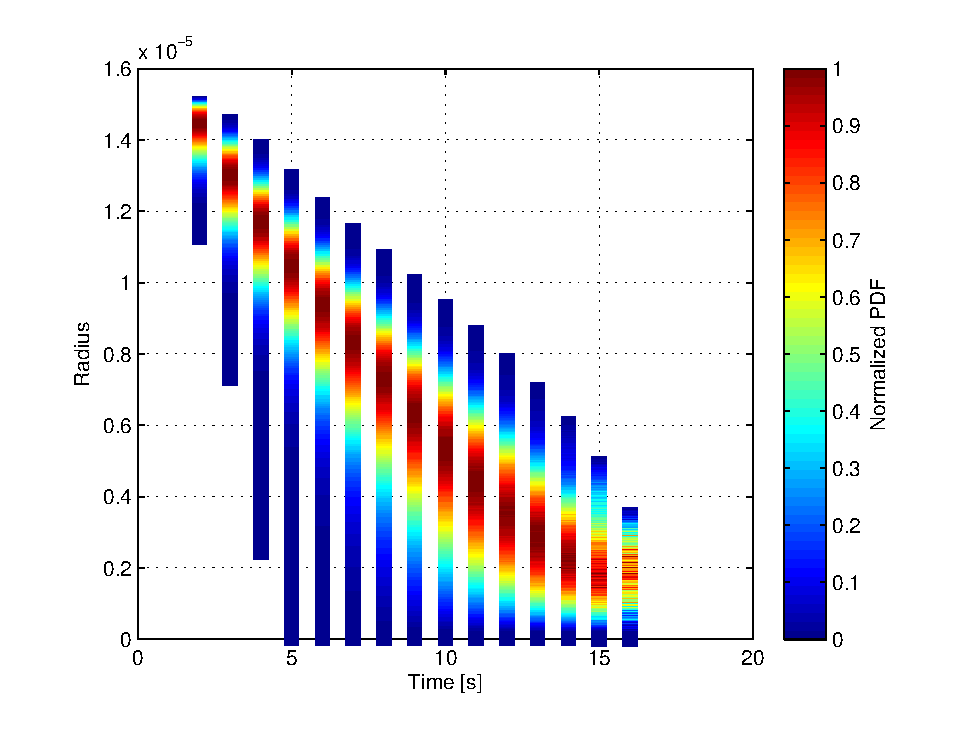
\includegraphics[width=0.48\textwidth]{Figures/pdf_radius_f1}\\
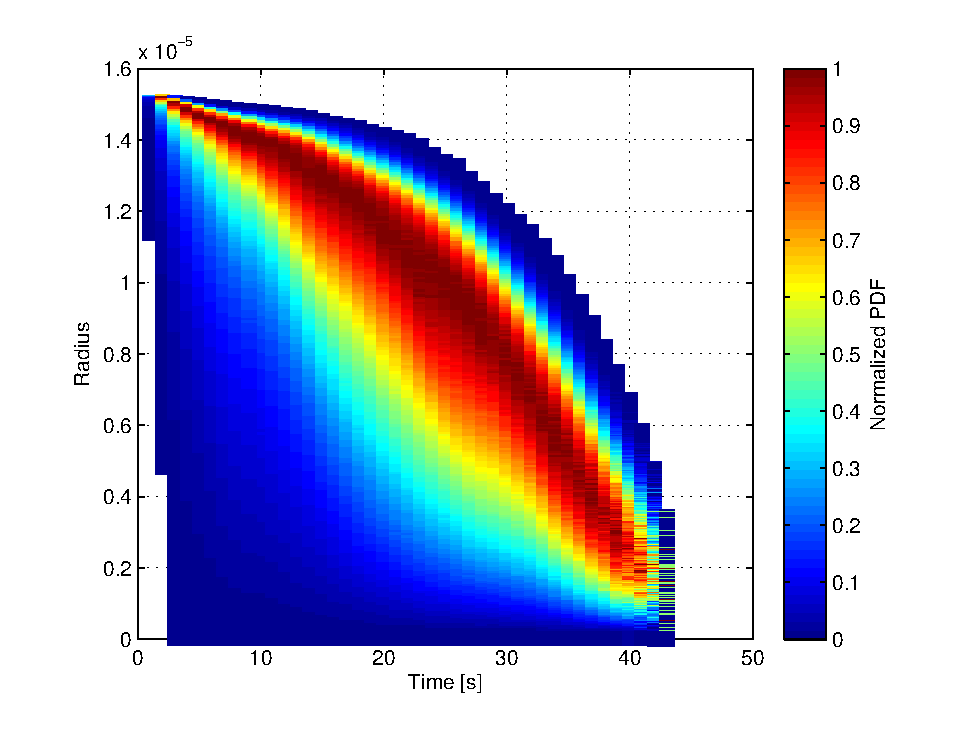
\includegraphics[width=0.48\textwidth]{Figures/pdf_radius_d2}
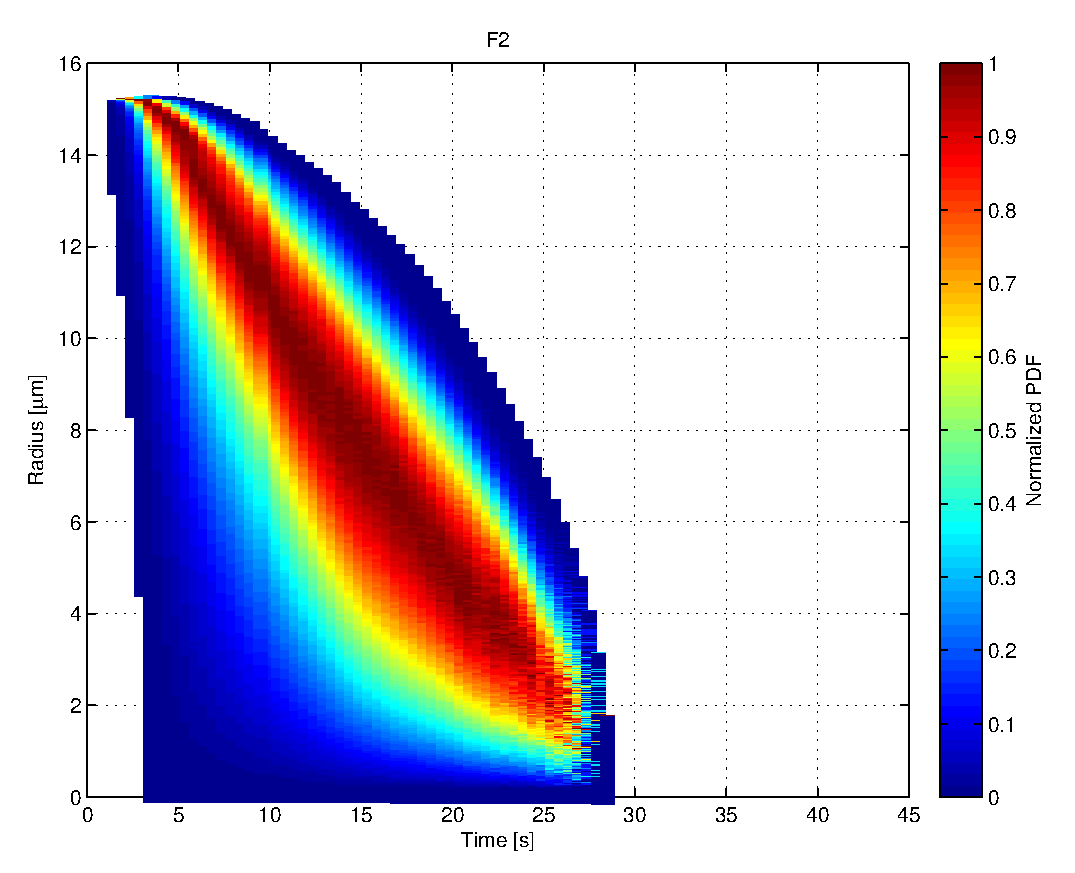
\includegraphics[width=0.48\textwidth]{Figures/pdf_radius_f2}\\
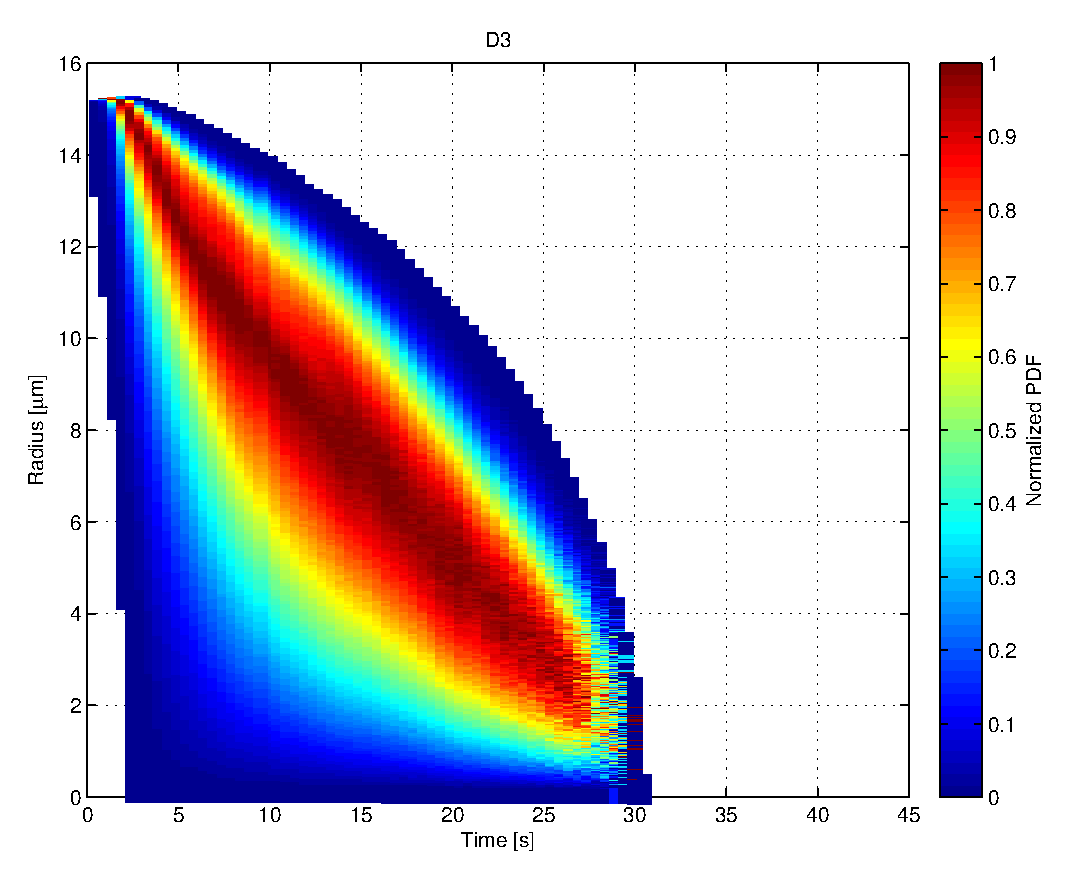
\includegraphics[width=0.48\textwidth]{Figures/pdf_radius_d3}
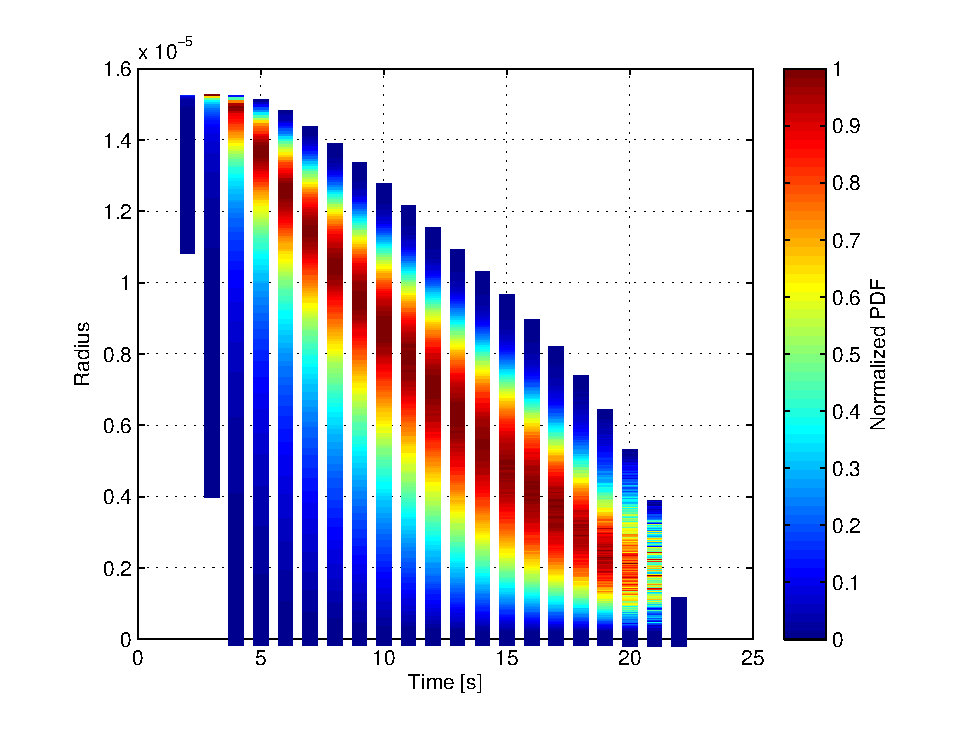
\includegraphics[width=0.48\textwidth]{Figures/pdf_radius_f3}
\caption{Evolution of radius distribution for decaying turbulence (left column) 
and forced turbulence (right column). From up to bottom are case 1, case 2 and case 3 respectively.}\label{fig:rad_distri}
\end{figure}

The distribution of supersaturation in \Fig{fig:supersat_distri} also clearly reflects the mixing process. Firstly, all the droplets stay in the cloud filaments thus has narrow spectrum and high probability density. After some droplets entering into the clear air, the spectrum immediately expands but with low probability density. This stage could be observed in D2 and D3, but extremely short for the rest cases. As mixing going on, the environment becomes much more homogeneous, that is most droplets stay in a similar environment. Finally, the environment becomes well-mixed, droplets completely evaporate and all the cases reach the same state.
\begin{figure}[H]
\includegraphics[width=0.48\textwidth]{Figures/pdf_supersat_d1}
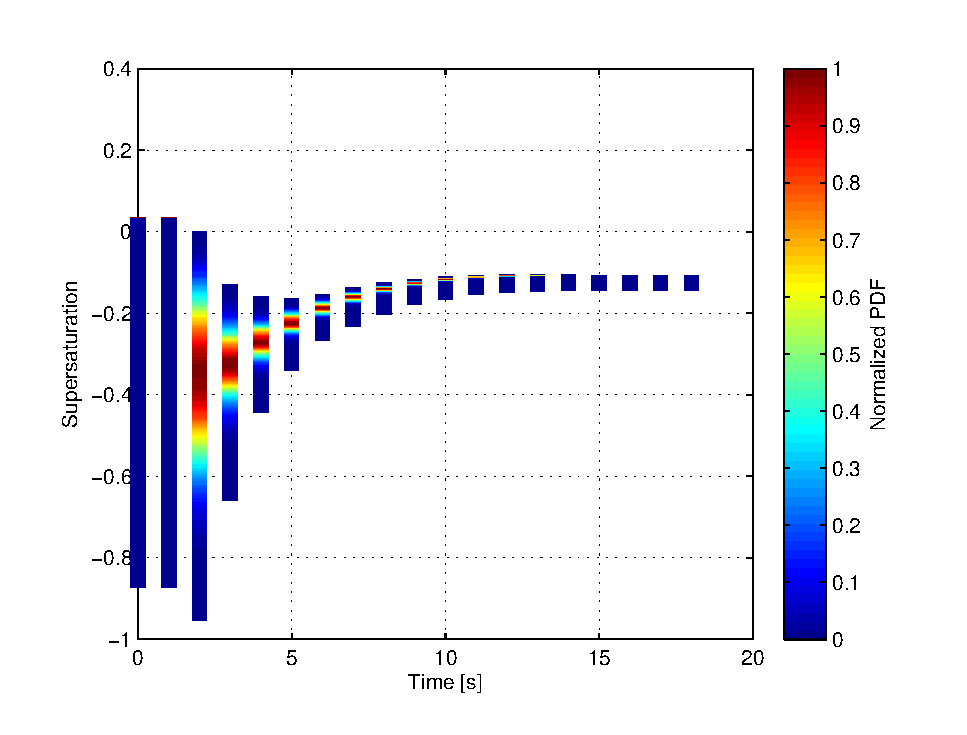
\includegraphics[width=0.48\textwidth]{Figures/pdf_supersat_f1}\\
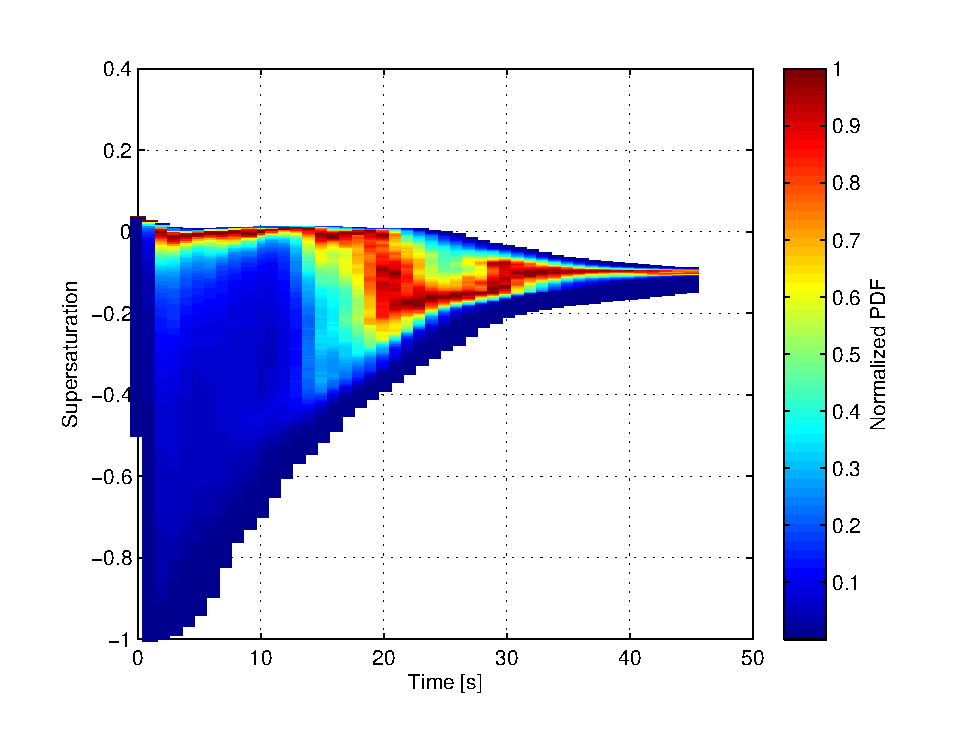
\includegraphics[width=0.48\textwidth]{Figures/pdf_supersat_d2}
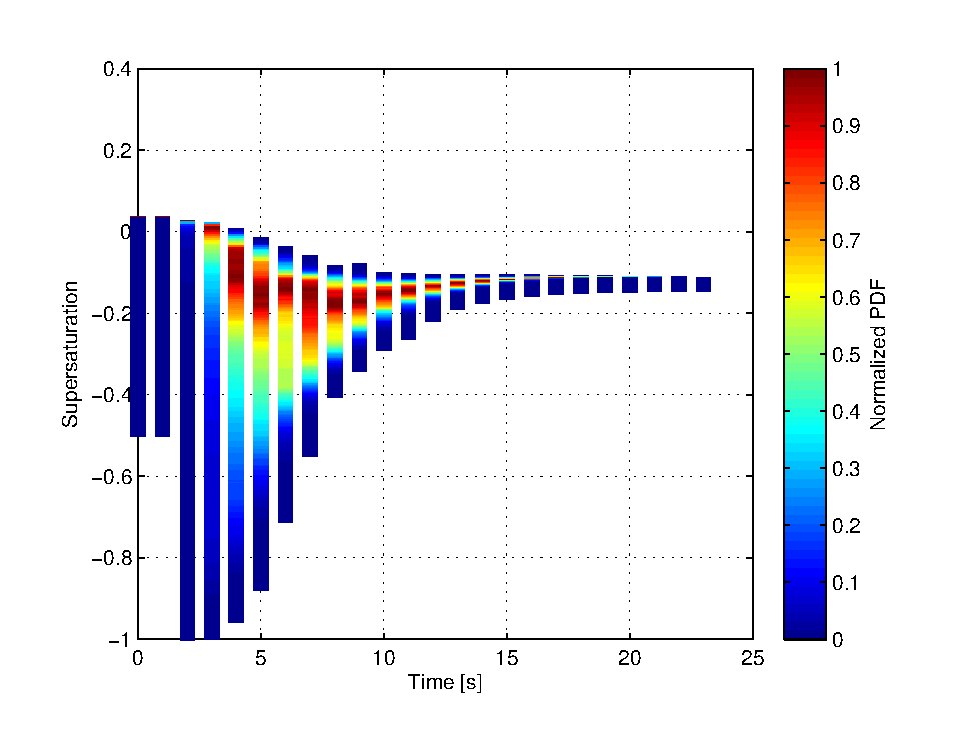
\includegraphics[width=0.48\textwidth]{Figures/pdf_supersat_f2}\\
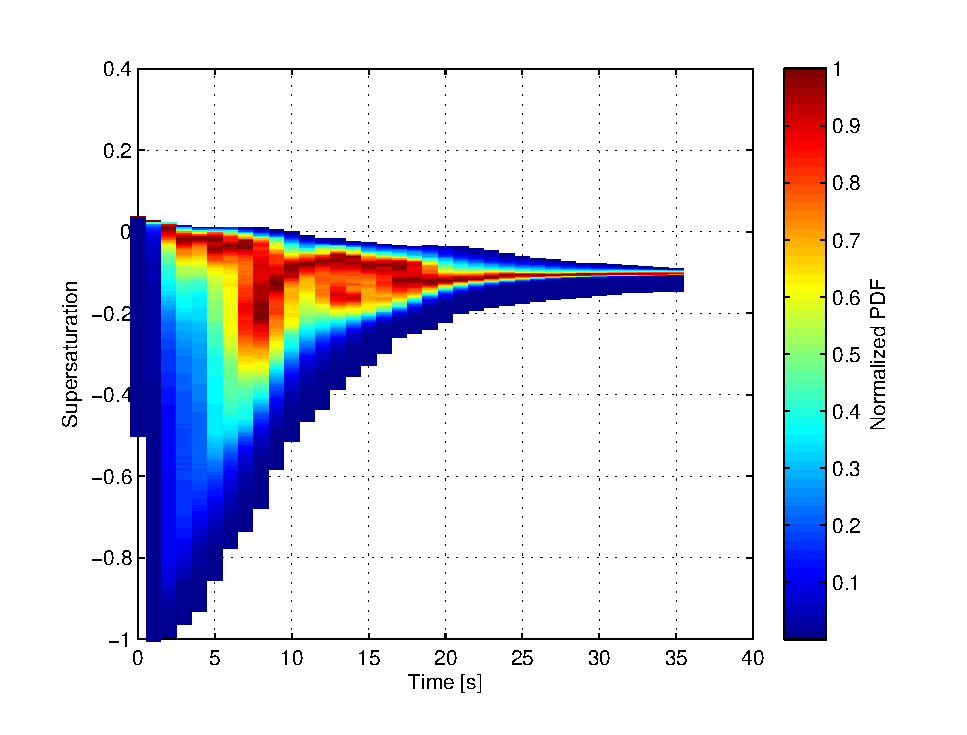
\includegraphics[width=0.48\textwidth]{Figures/pdf_supersat_d3}
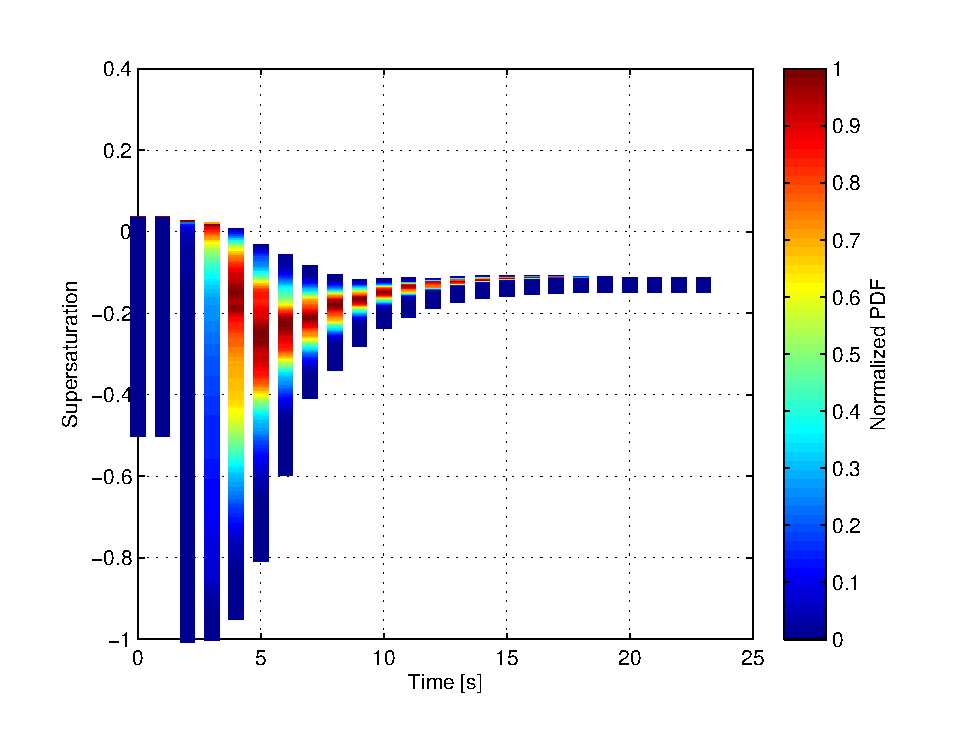
\includegraphics[width=0.48\textwidth]{Figures/pdf_supersat_f3}
\caption{Evolution of supersaturation distribution for decaying turbulence (left column) and forced turbulence (right column). From up to bottom are case 1, case 2 and case 3 respectively.}\label{fig:supersat_distri}
\end{figure}
In conclusion, the shape of the cloud filament has no influence on the final state after the mixing but will affect the intermediate process. The shape also has little impact on the mixing process for forced turbulence, while can not be completely ignored in the decaying cases. The results suggest that the initial shape of cloud filaments should be considered as an important factor when studying mixing scenario without external forcing.
\bibliographystyle{plain}
\bibliography{refs}

%\end{article}
\end{document}
